\section{Method}
\begin{figure}  
	% \advance\leftskip-1cm 
	\centering
	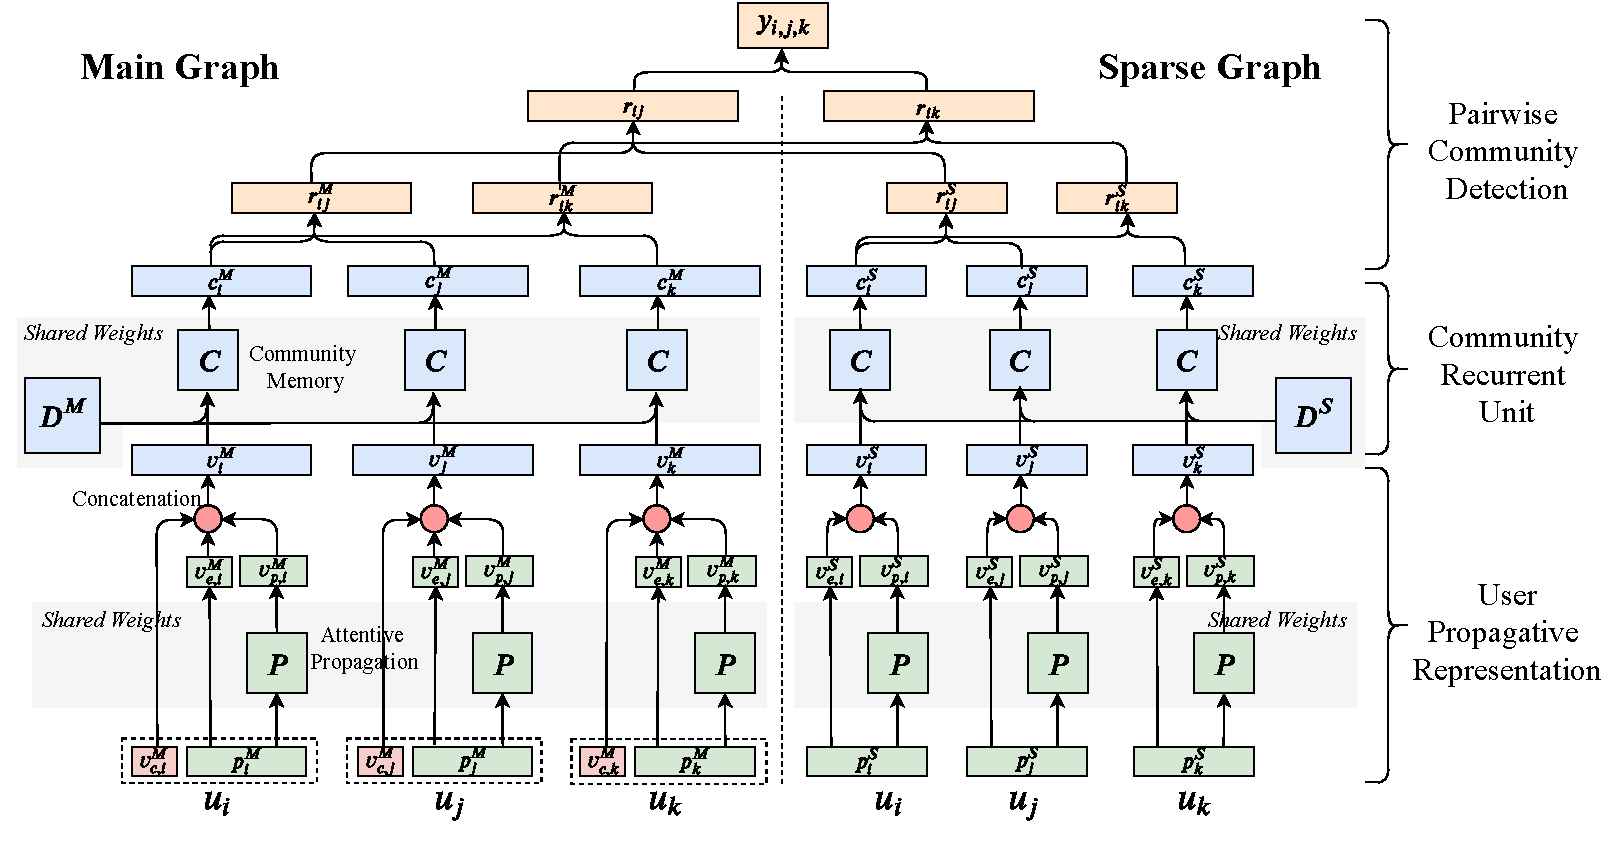
\includegraphics[width=1\columnwidth]{img/chapter4/pipeline.pdf}
	%  \vspace{-3em}
	\caption{The overall architecture of my proposed PCCD model. It contains three major modules mentioned in the right part of the figure. Each training instance is a mutual user triplet $\langle u_i,u_j,u_k \rangle$. Compared with the sparse graph, the main graph involves raw user community as part of model input.}
	
	\label{fig:c4_pipeline}
	%  \vspace{-1em} 
\end{figure}
\subsection{Task Overview} \label{sc:to}


As aforementioned, conventional methods suffer from graph sparseness problem. In this study, I propose a Pairwise Cross-graph Community Detection (PCCD) model that particularly aims at detecting user pairwise community closeness in sparse graphs by involving cross-graph techniques. 

Particularly, a well connected graph is called ``main graph" in this paper, corresponding to the targeted sparse graph. In general, as users may visit multiple cyber domains within a short time period, these mutual users co-occurred in both the main and sparse graph are taken as the bridge to connect the two graphs. Therefore, the relevant information from the main graph can be propagated to the sparse graph to support its user community detection. 

Specifically, my proposed model (showed in Figure \ref{fig:c4_pipeline}) is trained on mutual user triplets to learn three types of pairwise community relationship including ``\textit{similar}'', ``\textit{closer}'' and ``\textit{farther}''. The goal of this study can be reformulated as the following pairwise learning task: Given a sparse graph $S$ and a main graph $M$ where $N^C$ denotes their mutual user collection, for a mutual user triplet $\langle u_i,u_j,u_k \rangle  \in N^C$ (\textbf{Model Input}),  I aim to predict the relationship of its pairwise community closeness in graph $S$ (\textbf{Model Output}). In this paper, ``\textit{similar}'' relationship means that $u_j$ and $u_k$ are either in the same community or different communities with $u_i$. ``\textit{closer}'' relationship means that $u_j$ and $u_i$ are in the same community, while $u_k$ and $u_i$ are in different communities. ``\textit{farther}'' relationship means that $u_j$ and $u_i$ are in different communities, while $u_k$ and $u_i$ are in the same community.

For a mutual user triplet, my proposed model detects communities firstly on separate graphs to obtain all user raw community representations (Section \ref{sc:rcr}). Their propagative representations are learned through a community-level and a node-level filter (Section \ref{sc:upr}). Both representations are jointly utilized for predicting user community affiliation in each graph via a Community Recurrent Unit (Section \ref{sc:cru}). In the end, I integrate the community affiliation distributions to identify the pairwise community relationship of the triplet (Section \ref{sc:pcd}). Particular training strategies are introduced in the end (Section \ref{sc:mt}).

Note that even though my model is only trained on mutual users, it is still functional to detect pairwise community closeness on those users solely appeared in either the main or sparse graph. Further experiments in Section \ref{sc:ua} will verify its effectiveness on different types of users.

\subsection{Raw Community Representation} \label{sc:rcr}

As the user behavior is enriched in the main graph $M$, detecting user communities in it would offer auxiliary community features to potentially enhance my model performance. Therefore, I decide to involve user communities in the main graph as a part of model input. The same information from the sparse graph is intentionally omitted because its sparse graph structure is not able to offer reliable community partition results.

Considering all possible community detection methods listed in Section \ref{sc:baseline}, Infomap is empirically selected to detect user communities in the main graph $M$. Infomap method simulates a random walker wandering on the graph for $m$ steps and indexes his random walk path via a two-level codebook. Its final goal aims to generate a community partition with the minimum random walk description length, which is calculated as follows:

\begin{equation} 
\textit{$L(\pi)$} = \sum_{i}^{m}q_{\curvearrowright}^{i}H(\mathcal{Q})+\sum_{i=1}^{m} \textit{$p_{\circlearrowright}^{i}$}H(\textit{$\mathcal{P}^{i}$}) 
\end{equation}
where \textit{$L(\pi)$} is the description length for a random walker under current community partition $\pi$. $q_{\curvearrowright}^{i}$ and $p_{\circlearrowright}^{i}$ are the jumping rates between communities and within the $i_{th}$ community in each step. $H(\mathcal{Q})$ is the frequency-weighted average length of codewords in the global index codebook and $H(\mathcal{P}^{i})$ is frequency-weighted average length of codewords in the $i_{th}$ community codebook.


In the end, given a user $u_i$, I obtain its one-hot community representation $v_{c,i}^M$ in the main graph $M$, which is regarded as part of user representations for the model input.

\subsection{User Propagative Representation}\label{sc:upr}


\begin{figure}  
	% \advance\leftskip-1cm 
	\centering
	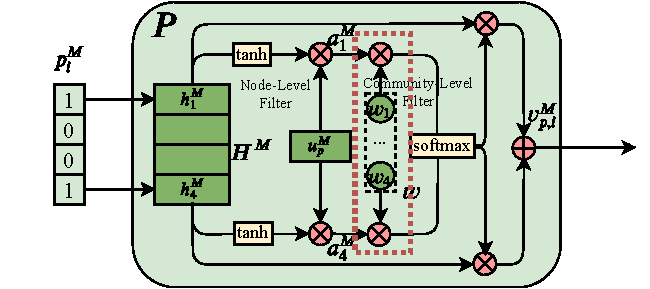
\includegraphics[width=\columnwidth]{img/chapter4/propagation.pdf}
	% 	\vspace{-1em}
	\caption{The two-level filter to support user propagative representation estimation in the main graph $M$. Sparse graph $S$ does not contain the community-level filter ( wrapped in the red rectangle).}
	\label{fig:propagation}
	% 	\vspace{-1.5em} 
\end{figure}

To better convey the mutual user insights in both main and sparse graph, their representations are learned from both direct transformation and weighted information propagation. The optimization processes are similar in the main and sparse graph. In the beginning, a user $u_i$ can be represented as a multi-hot embedding $p_{i}^{M}$ in the main graph $M$ (left part in Figure \ref{fig:propagation}) and $p_{i}^{S}$ in the sparse graph $S$. Each dimension in the embedding refers to a unique object with which the user connects in the related graph. 

The direct transformation from user multi-hot embedding learns a dense vector via one hidden layer so as to retrieve the compressed  information from user connected objects directly, which is calculated as follows:

\begin{equation}
v_{e,i}^{G} = {\rm tanh}(W_e^Gp_i^G + b_e^G) 
\end{equation}

where $G \in \{M, S\}$ denotes either the main or the sparse graph. $W_e^G$ and $b_e^G$ denote the weight matrix and bias respectively. $v_{e,i}^{G}$ is the learned direct transformation representation for user $u_i$.

On the other hand, from information propagation perspective, each object carries information, which can be propagated to its connected users as a type of representation. However, as such information are noisy and heterogeneous, not all of them are equally important to users. Therefore, a filtering module is proposed to automatically select appropriate information to propagate from both community level and node level.  The overall flow of the filtering module is illustrated in Figure \ref{fig:propagation}.

\textbf{Community-Level Filter:} As the raw detected communities in the sparse graph is not reliable because of graph sparseness, I only apply the community-level filter in the main graph $M$. According to the raw community partition $\pi$ calculated in Section \ref{sc:rcr}, each object node $n_i$ is assigned to a community $\pi(n_i)$. The community-level filter propagate object information in a coarser manner by considering its community importance weight $w_{\pi(n_i)}$. Throughout this filter, I aim to learn a weight vector $w$ where each dimension of $w$ denotes the importance score of a related community. 


\textbf{Node-Level Filter:} Node-level filter assesses the propagated information with a fine resolution. In the main graph $M$ ( a user-object bipartite graph), I aim to learn object representations $H^M = \{h_1^M,...,h_n^M\}$ where $h_n^M$ denotes the $n_{th}$ object representation. Similarly, $H^S$ denotes the object representations in the sparse graph $S$. The weight of the $j_{th}$ object node decides the amount of its information propagating to its connected user nodes, which is calculated in an attentive means: 

\begin{equation} \label{eq:np}
a_{j}^{G} = (u_p^{G})^{\intercal} {\rm tanh}(W^{G}_p h_{j}^{G} +b_p^{G})
\end{equation}

where $G \in\{M,S\}$ denotes either the main or the sparse graph. $u^{G}_p$ denotes the project vector in the related graph to calculate object attentive weights. $W_p^{G}$ and $b_p^{G}$ denote the corresponding weights and bias, respectively. 

I combine the community-level and node-level weights together to quantify the information propagation in the main graph $M$. While only the node-level weights is considered in the sparse graph $S$. Normalized by the ${\rm softmax}(\cdot)$ function, the related representation of  user $u_i$ in both graphs are calculated as follows:
\begin{equation}\label{eq:pv}
\begin{aligned} 
& v_{p,i}^{M} = \sum_{n_j \in \mathcal{N}^{M}(u_i)} {\rm softmax}(a_{j}^{M} w_{\pi(n_j)})  h_{j}^{M} \\
& v_{p,i}^{S} = \sum_{n_j \in \mathcal{N}^{S}(u_i)}{\rm softmax}(a_{j}^{S}) h_{j}^{S} 
\end{aligned} 
\end{equation}

Both $v_{p,i}^{M}$ and $v_{p,i}^{S}$ are the weighted sum of the neighbour object representations. $\mathcal{N}^{S}(n_i)$ and $\mathcal{N}^{M}(n_i)$ denote user connected objects in both graphs. 

Finally, given a user $u_i$, its raw community representation, direct transformation representation and two-level filtered representation construct its propagative representation in the main graph $M$. While its direct transformation representation and node-level filtered representation construct its propagative representation in the sparse graph $S$. To avoid gradient vanishing, a ${\rm batch\_norm(\cdot)}$ function is applied on top of the concatenated representations in both graph:
\begin{equation} \label{eq:nv}
\begin{aligned} 
& v_{i}^{M} = {\rm batch\_norm}([v_{c,i}^{M},v_{e,i}^{M},v_{p,i}^{M}]) \\
& v_{i}^{S} = {\rm batch\_norm}( [v_{e,i}^{S},v_{p,i}^{S}])
\end{aligned} 
\end{equation} 

\subsection{Community Recurrent Unit}\label{sc:cru}

After previous steps, each user of the mutual user triplet $\langle u_{i},u_{j},u_{k}\rangle$ is associated with a propagative representation. In this section, its corresponding community affiliation scores $c_{i}^{G}$ are further calculated in related graphs $G \in\{M,S\}$ through a designed Community Recurrent Unit (CRU), which is showed in Figure \ref{fig:cru}. The CRU contains an affiliation gate to calculate the user affiliation score for each community and an update gate to update community self representations. Within this unit, a community memory $D^{G} = \{d_1^G,...,d_K^G\}$ is designated to store $K$ community representations. Particularly, community representation is required to be with the same dimension as user propagative representation in both graphs.
\textbf{Community Affiliation Gate:} The affiliation gate helps to generate the affiliation score of a user $u_i$ towards each community in both graphs, which forms a $K$-dimensional vector $c_{i}^{G} = \{c_{i,1}^{G},...,c_{i,K}^{G}\}$ where $G \in \{M, S\}$ . The user $u_i$'s affiliation score $c_{i,j}^G$ towards the $j_{th}$ community in the graph $G$ is calculated as follows:

\begin{equation}\label{eq:dg}
c_{i,j}^G = {\rm  \sigma}((u_{c}^{G})^{\intercal}({\rm  tanh}(v_{i}^{G})*d_j^G))
\end{equation}

The dot product between transformed user propagative representation ${\rm  tanh}(v_{i}^{G})$ and the $j_{th}$ community representation $ d_j^G$ indicates their potential correlation, which further  turns to a scalar affiliation score $c_{i,j}^G$ between 0 to 1 with the help of a projection vector $u_{c}^{G}$ and normalization function $\sigma(\cdot)$.

\begin{figure}  
	% 	\advance\leftskip-2cm 
	\centering
	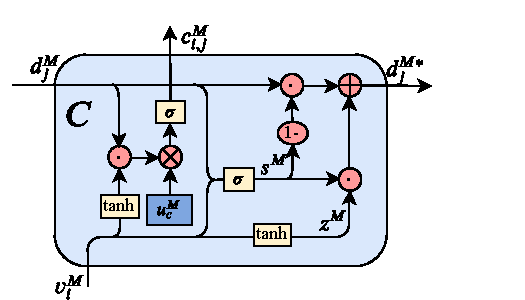
\includegraphics[width=1.2\columnwidth]{img/chapter4/cru.pdf}
	% 	\vspace{-1em}
	\caption{The flow of Community Recurrent Unit in the main graph $M$. The left part refers to the community affiliation gate and the right part is the community update gate.}
	\label{fig:cru}
	% 	\vspace{-1.5em} 
\end{figure}

\textbf{Community Update Gate: } \label{sc:cug} When calculating $u_i$'s community affiliation, its information can help to update community representations in return. The updated representation is relied on both previous step community representation and current user propagative representation. Therefore, to better embrace the two representations, I use a delicate RNN variant, where the update process is calculated as follows:

\begin{equation}\label{eq:up}
\begin{aligned}
&  s^G = \sigma(W_s^G[v_i^{G},d_j^{G}] + b_s^G) \\
& z^G = {\rm tanh}(W_z^Gv_i^G+b_z^G)\\
& d_j^{G*} = (1-s^G)*d_j^{G} + s^G*z^G
\end{aligned}
\end{equation}

where $G \in \{M,S\}$. $s^G$ denotes the update rate and $z^G$ is transformed user information to be updated in current community.  $d_j^{G*}$ denotes the updated representation of the $j_{th}$ community in graph $G$, which is the weighted sum on previous community and current user representations. $W_s^G$ and $W_z^G,$ denote related weight matrices, while $b_s^G$ and $b_z^G,$ denote related biases. 

\textbf{Community Constraint: }
To obtain the communities with less overlapping information in graph $G \in \{M,S\}$, the community representations ideally should be independent with each other. In my model, cosine similarity ${\rm cos}(\cdot)$ is taken as the criteria to measure the community similarity where higher score indicates stronger correlation. The averaged cosine similarities of all possible community representation pairs is calculated as a community loss to minimize:

\begin{equation}\label{eq:cc}
\mathcal{L}_{c}^{G} = \frac{1}{2K^2}\sum_{i,j}{\rm cos}(d_i^{G},d_j^{G})
\end{equation}
where $K$ is the number of communities in each graph.

\subsection{Pairwise Community Detection}\label{sc:pcd}

Similar to RankNet \cite{burges2010ranknet}, given a mutual user triplet  $\langle u_i,u_j,u_k \rangle$, as three types of pairwise label are considered including ``\textit{closer}'', ``\textit{similar}'' and ``\textit{farther}'', label $y_{i,j,k}$  is calculated as follows:
\begin{equation}\label{eq:y}
y_{i,j,k} = \frac{1}{2}(1+S_{jk})
\end{equation}
In terms of the community closeness for $u_i$, if $u_j$ is closer than $u_k$, $S_{jk} = 1$; if $u_j$ is farther than $u_k$, $S_{jk} = -1$; if $u_j$ and $u_k$ are similar, $S_{jk} = 0$. In this way, I convert the pairwise ranking task to a regression task. 

To optimize this task, first of all, I calculate the correlation representation $r^{G}_{ij}$ between $u_j$ and $u_i$ in single graph $G \in \{M,S\}$:

\begin{equation}\label{eq:gr}
r^{G}_{ij} = W^{G}_{r}(c_{i}^{G} - c_{j}^{G}) +  b^{G}_{r} 
\end{equation}

where $ W^{G}_{r}$ and $ b^{G}_{r}$ are related weight and bias, respectively. 

To construct the information from both graphs, I concatenate the correlation representations from both graphs:
\begin{equation} \label{eq:cr}
r_{ij} = {\rm tanh}([r^{S}_{ij},r^{M}_{ij}])
\end{equation}
Similarly, the cross-graph correlation representation  between $u_i$ and $u_k$ is calculated as $r_{ik}$. 

After that, I predict the community relationship between $u_j$ and $u_k$ towards $u_i$ as follows:
\begin{equation} \label{eq:yp}
\hat{y}_{i,j,k} = \sigma(W_{o}(r_{ij} - r_{ik}) +  b_{o})
\end{equation}

where $W_{o}$ and $b_{o}$ are the related weight and bias. $\sigma(\cdot)$ denotes the sigmoid activation function. In the end, the final loss $\mathcal{L}_{total}$ is the weighted sum of the optimization loss calculated via cross entropy and the community constraint losses where  $\mathcal{L}_{c}^S$ is for the sparse graph and $\mathcal{L}_{c}^M$ is for the main graph:
\begin{equation}\label{eq:loss}
\mathcal{L}_{total} = \underbrace{-y_{i,j,k}log\hat{y}_{i,j,k}-(1-y_{i,j,k})log(1-\hat{y}_{i,j,k})}_{optimization} + \underbrace{\alpha(\mathcal{L}_{c}^S + \mathcal{L}_{c}^M)}_{constraint}
\end{equation}

\subsection{Training Strategy}\label{sc:mt}

Although my model is trained solely on mutual user triplets, it is also able to detect pairwise community closeness among users only appeared in either sparse graph or main graph. Two training tricks are particularly employed in my model to improve model robustness, including shared weights and masked training. 

First, as my model should be insensitive to the sequence of input user triplet, the weight matrices, biases and project vectors in both Section \ref{sc:upr} and Section \ref{sc:cru} should be shared among the three users. Moreover, in  Section \ref{sc:cru}, the community memory $D^G$ where $G \in \{M,S\}$ is updated by taking the average of the three updated community representations (calculated in Eq. \ref{eq:up}) from input triplets.

Second, to alleviate the negative effects of excessive connections in main graph $M$, I employ a masked training strategy by randomly remove a small ratio $\rho$ of connected objects from users in the main graph during each training batch. $\rho = 0$ means users remain their original multi-hot embeddings while $\rho = 1$ means users lose all their connections on objects. 




